\documentclass[12pt,letterpaper,titlepage]{article}
\usepackage{solarized-light}
\usepackage{fontspec}
\defaultfontfeatures{Mapping=tex-text}
\usepackage{xunicode}
\usepackage{xltxtra}
\usepackage{amsmath}
\usepackage{pdfpages}
\usepackage{amsfonts}
\usepackage{amssymb}
\setcounter{secnumdepth}{0}
\usepackage{nameref}
\usepackage{enumitem}
\usepackage{environ}
\usepackage{pdfpages}
\usepackage{pgfplots}
\usepackage{karnaugh-map}

\setmainfont{Times New Roman}
\showboxdepth=\maxdimen
\showboxbreadth=\maxdimen


\usepackage{paracol}
\usepackage{wrapfig}
\globalcounter{table}
\globalcounter{figure}
\usepackage{graphicx}
\usepackage[left=1in,right=1in,top=1in,bottom=1in]{geometry}
\graphicspath{{img/}}

\author{Jacob Abel}
\title{	Project 3A
	\\\large ECE3544 CRN:82989
}

\setlength{\parskip}{0.25em}

\begin{document}
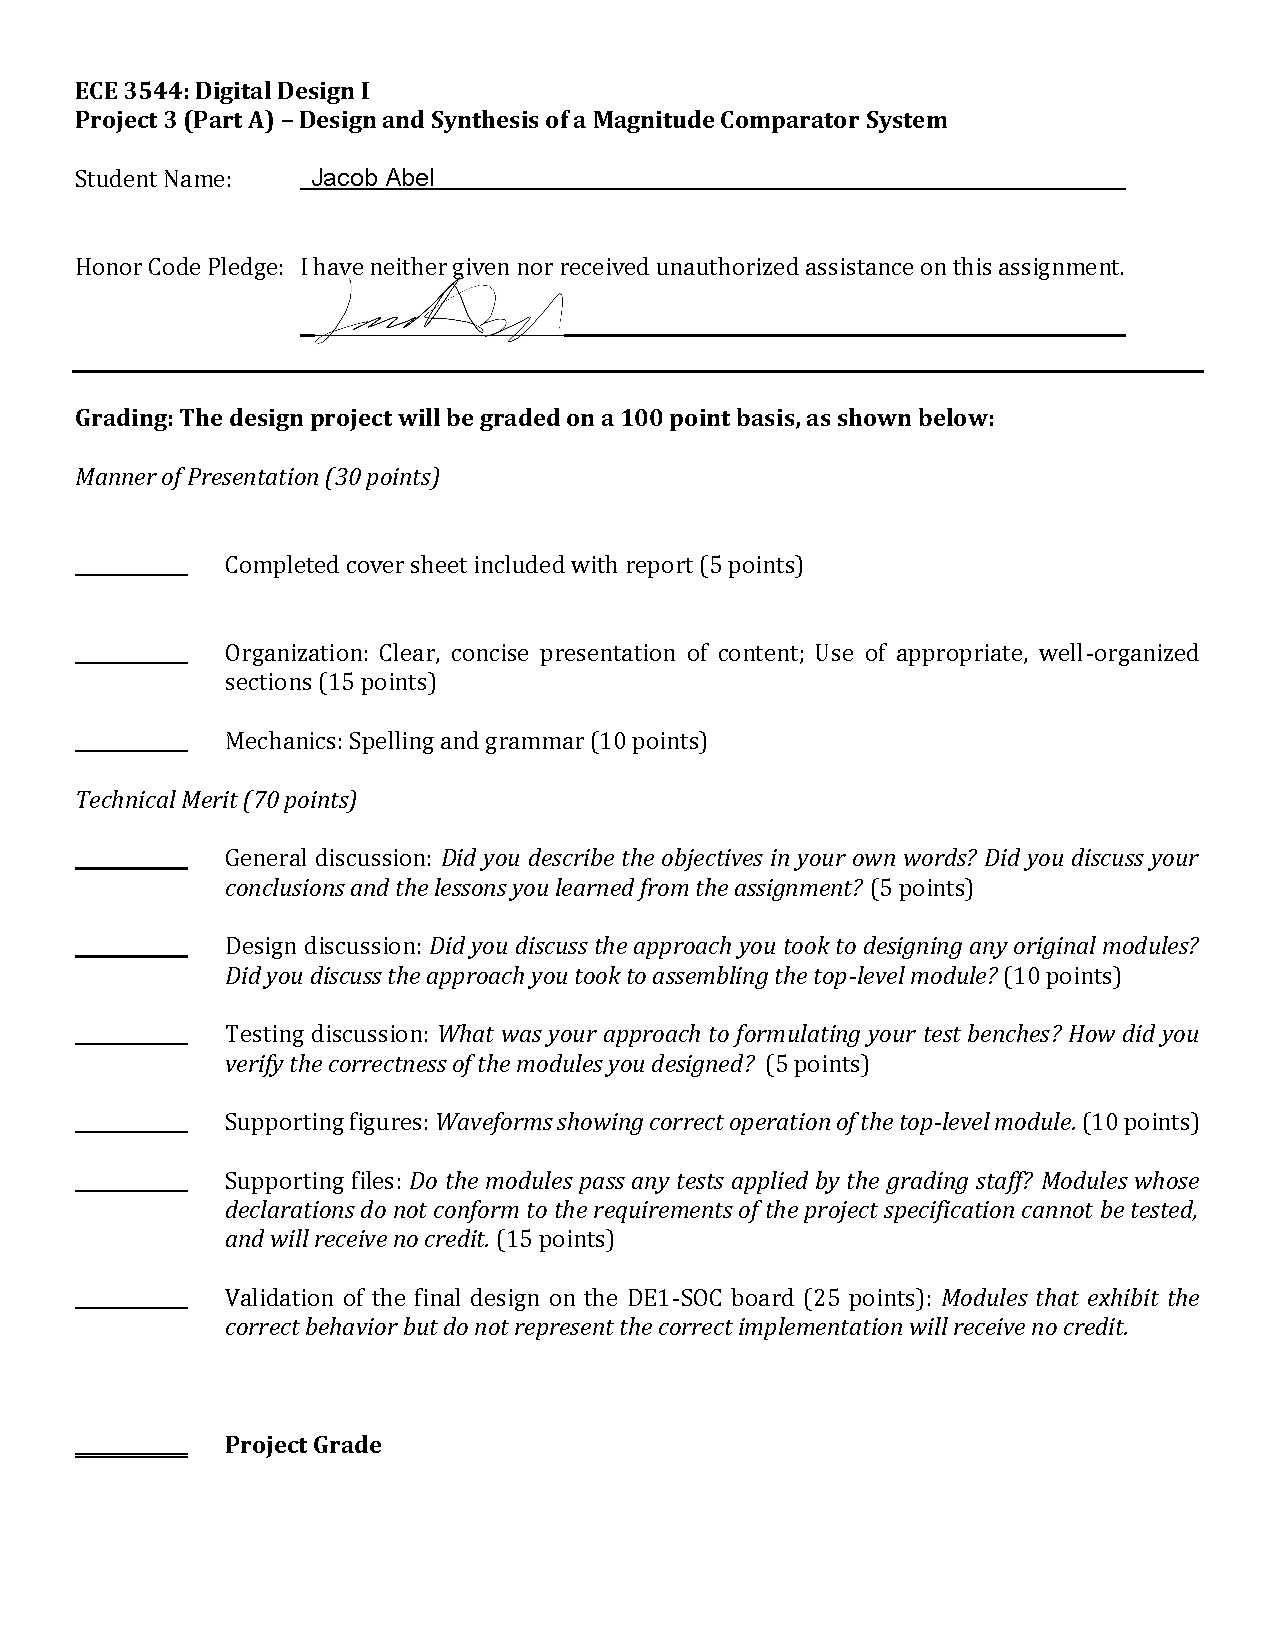
\includepdf[noautoscale]{CoverSheet.pdf}
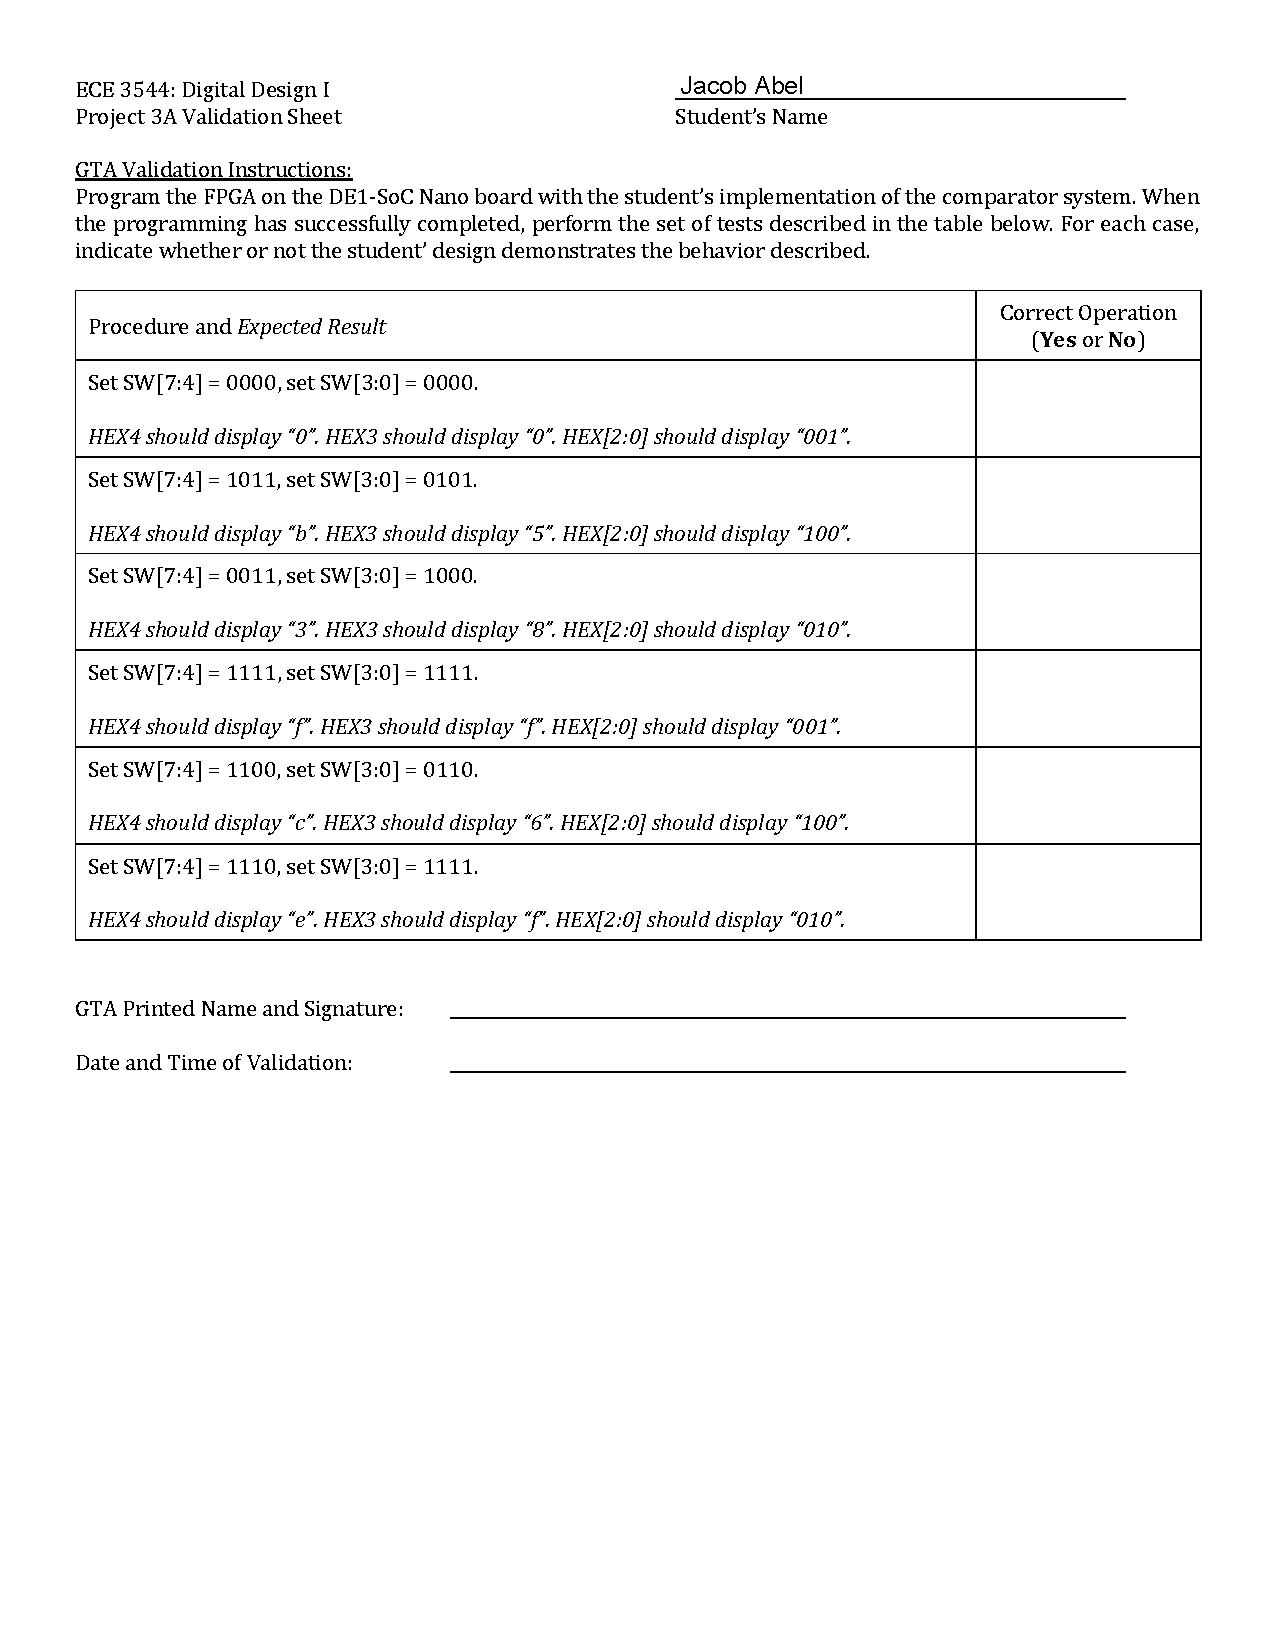
\includepdf[noautoscale]{ValidationSheet.pdf}

\maketitle
\begin{raggedright}

\section*{Objective}
The objective of this project is to demonstrate a capability to synthesise designs onto a real world system such as an FPGA and produce the same output as the simulated designs. Additionally, this project demonstrates basic competence utilising the Quartus IDE.

\section{Module Design}
The design process was rather straight forward. The pins were matched with the corresponding values using the manual. Once the board was functioning and designs were exportable, the module was implemented. As it was relatively straightforward, an enable bit was added to the hc85 module along with some self explanatory dataflow Verilog and the primary module was implemented using structural Verilog. The test bench was more or less a reimplementation of the hc85 test bench with some slight modifications. The 7-segment display driver module had previously been designed with a corresponding test bench. The entire module is essentially a large case block containing each possible display value and was a trivial design.

Once the primary module was implemented, the test bench was checked and the equivalence bit suggested that the design was functional. At this point the design was synthesised and the same tests as in the test bench were run on a DE1 board.

\clearpage
\section{ECE3544Project3a Module Simulation}
\begin{center}
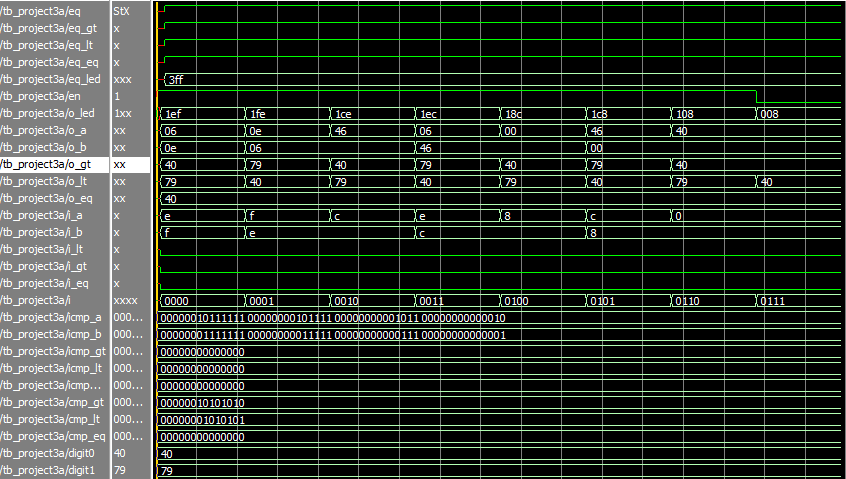
\includegraphics[width=\textwidth]{tb_p3a}

\end{center}

This simulation demonstrates that all the basic inputs produce the correct outputs. The \texttt{en} and \texttt{i\_} values are the inputs that compose the switch input values and the \texttt{o\_} values are the outputs as 7 segment display values. The \texttt{eq\_} wires demonstrate equivalence on each output pin and the \texttt{eq} wire demonstrates equivalence on all outputs. The equivalences are computed using an XNOR against expected results.

\section{Conclusion}

This project demonstrated the equivalence of Verilog simulations and real world FPGA module synthesis. Despite starting this project late, the project went remarkably smoothly and very little of the time was spent debugging. As such the project can easily be considered a success with the exception of the scheduling failure that resulted in it being started late.

\end{raggedright}
\end{document}
